\documentclass[a4paper]{article}



%% Sets page size and margins
\usepackage[a4paper,top=2cm,bottom=2cm,left=3cm,right=3cm,marginparwidth=1.75cm]{geometry}

%% Useful packages
\usepackage{amsmath,amsthm,amssymb,amsfonts,graphicx, fancyvrb}
\usepackage{drawstack}

\title{\vspace{-1.5cm}IERG4130 Assignment 2}

\author{LAU Long Ching\\SID: 1155127347\\
        
}

\date{16/03/2021}



\begin{document}
\maketitle
\section*{Question 1}
The only prime number factors for n=35 is p=7 and q=5.\\\\
$\textrm{z} = (\textrm{p}-1)(\textrm{q}-1) = 24$\\\\
Since e=5, $5\times \textrm{d} \textrm{ mod } 24 = 1$\\\\
The private key can be (d=29, n=35).\\\\
$M = C^d \textrm{ mod } n = 11^{29} \textrm{ mod } 35 = 16$.

\section*{Question 2}
The only prime number factors for n=34163 is p=127 and q=269.\\\\
$\textrm{z} = (\textrm{p}-1)(\textrm{q}-1) = 33768$\\\\
Since e=5, $5\times \textrm{d} \textrm{ mod } 33768 = 1$\\\\
The private key can be (d=54029, n=34163).

\section*{Question 3}
\subsection*{(a)}
Since we have the prime q=11 and the primitive root $\alpha$=2,\\\\
$2^{x} \textrm{ mod } 11 = 9$\\\\
We have Alice's secret key x=6.
\subsection*{(b)}
The shared secret key $ = 3^6 \textrm{ mod } 11 = 3$.
\pagebreak
\section*{Question 4}
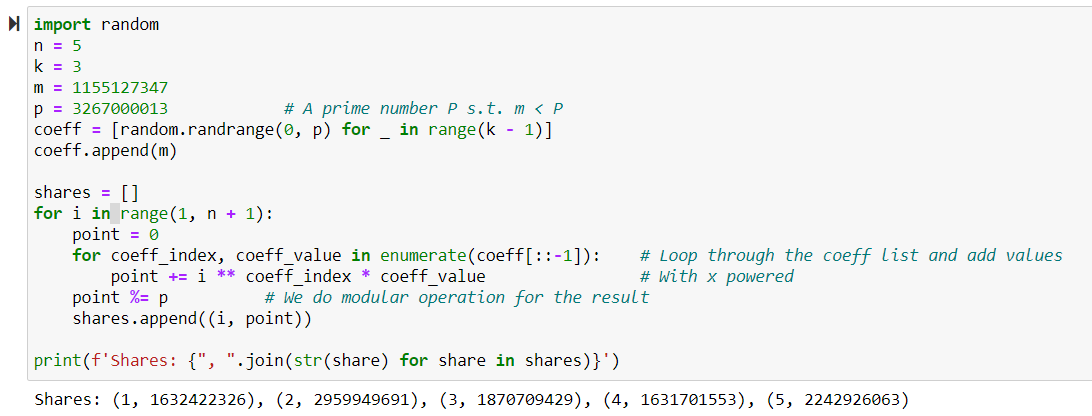
\includegraphics[scale=0.6]{1.png}\\\\
3 pairs of the key (1, 1632422326), (2, 2959949691), (3, 1870709429) would be enough for the decryption.\\\\
Please find the .py file attached. The source code can also be found above.

\section*{Question 5}
\subsection*{(a) (b)}
Please refer to attachments.
\subsection*{(c)}
The issuer of the certificate is called "Let's Encrypt". It also has a common name "R3".
\subsection*{(d)}
On crt.sh, we can find the public key of the issuer:\\\\
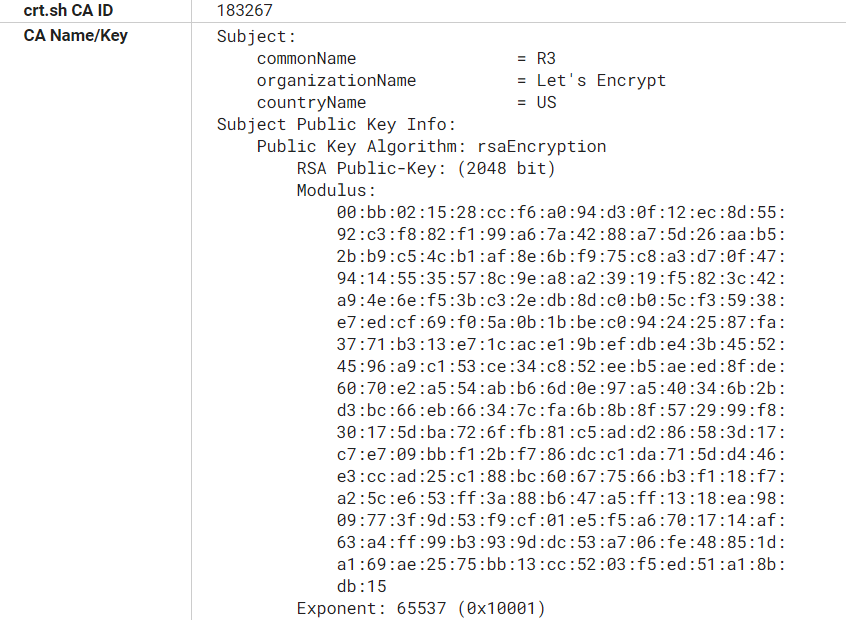
\includegraphics[scale=0.6]{3.png}
\pagebreak
\section*{Question 6}
\subsection*{(a)}
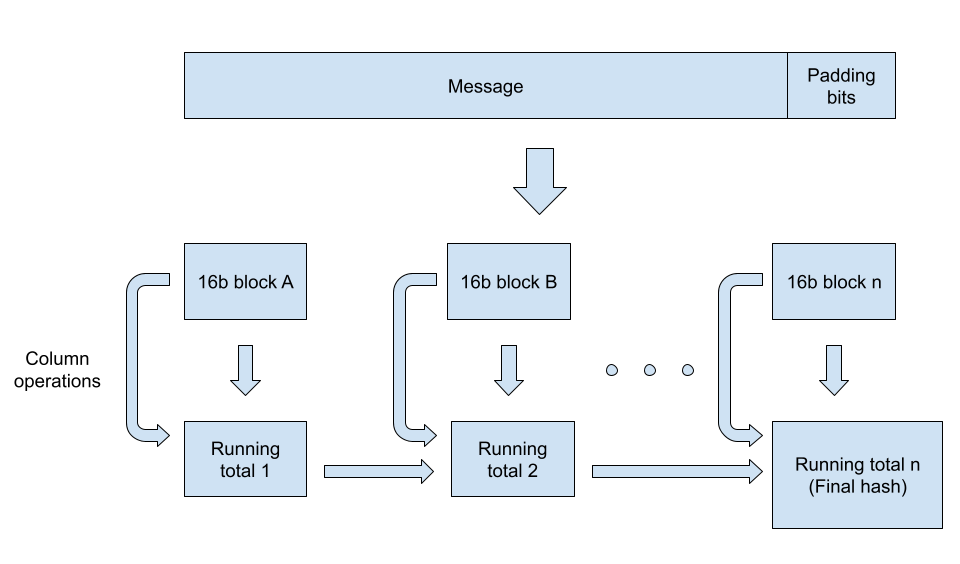
\includegraphics[scale=0.4]{2.png}
\subsection*{(b)}
First block:\\\\
\begin{tabular}{|l|l|l|l|}
\hline
A & L & I & C \\ \hline
E & T & H & I \\ \hline
N & K & S & T \\ \hline
H & E & A & S \\ \hline
\end{tabular}
\quad
converts to 
\quad
\begin{tabular}{|l|l|l|l|}
\hline
0 & 11 & 8 & 2 \\ \hline
4 & 19 & 7 & 8 \\ \hline
13 & 10 & 18 &19 \\ \hline
7 & 4 & 0 & 18 \\ \hline
\end{tabular}
\quad
after column operations
\quad
\begin{tabular}{|l|l|l|l|}
\hline
4 & 10 & 0 & 18 \\ \hline
13 & 4 & 8 & 19 \\ \hline
7 & 11 & 7 &8 \\ \hline
0 & 19 & 18 & 2 \\ \hline
\end{tabular}
\\\\\\Running total: $(0, 0, 0, 0) \rightarrow (21, 12, 8, 3) \rightarrow (1, 4, 15, 16)$\\\\\
Second block:\\\\
\begin{tabular}{|l|l|l|l|}
\hline
S & I & G & N \\ \hline
M & E & N & T \\ \hline
I & S & V & E \\ \hline
R & Y & E & A \\ \hline
\end{tabular}
\quad
converts to 
\quad
\begin{tabular}{|l|l|l|l|}
\hline
18 & 8 & 6 & 13 \\ \hline
12 & 4 & 13 & 19 \\ \hline
8 & 18 & 21 &4 \\ \hline
17 & 24 & 4 & 0 \\ \hline
\end{tabular}
\quad
after column operations
\quad
\begin{tabular}{|l|l|l|l|}
\hline
12 & 18 & 4 &0 \\ \hline
8 & 24 & 6 & 4 \\ \hline
17 & 8 & 13 &19 \\ \hline
18 & 4 & 21 & 13 \\ \hline
\end{tabular}
\\\\\\Running total: $(1, 4, 15, 16) \rightarrow (20, 0, 14, 9) \rightarrow (2, 16, 19, 13)$\\\\\
Third block:\\\\
\begin{tabular}{|l|l|l|l|}
\hline
S & Y & F & O \\ \hline
R & O & U & R \\ \hline
S & T & U & D \\ \hline
E & N & T & S \\ \hline
\end{tabular}
\quad
converts to 
\quad
\begin{tabular}{|l|l|l|l|}
\hline
18 & 24 & 5 & 14 \\ \hline
17 & 14 & 20 & 17 \\ \hline
18 & 19 & 20 &3 \\ \hline
4 & 13 & 19 & 18 \\ \hline
\end{tabular}
\quad
after column operations
\quad
\begin{tabular}{|l|l|l|l|}
\hline
17 & 19 & 19 &18 \\ \hline
18 & 13 & 5 & 3 \\ \hline
4 & 24 & 20 &17 \\ \hline
18 & 14 & 20 & 14 \\ \hline
\end{tabular}
\\\\\\Running total: $(2, 16, 19, 13) \rightarrow (11, 6, 1, 15) \rightarrow (6, 19, 14, 3)$\\\\\
The hash is GTOD.


\subsection*{(d)}
First block:\\\\
\begin{tabular}{|l|l|l|l|}
\hline
A & A & A & A \\ \hline
G & A & A & A \\ \hline
N & A & A & A \\ \hline
B & A & A & A \\ \hline
\end{tabular}
\quad
converts to 
\quad
\begin{tabular}{|l|l|l|l|}
\hline
0 & 0 & 0 & 0 \\ \hline
6 & 0 & 0 &0 \\ \hline
13 & 0 & 0 &0 \\ \hline
1 & 0 & 0 & 0 \\ \hline
\end{tabular}
\quad
after column operations
\quad
\begin{tabular}{|l|l|l|l|}
\hline
6 & 0 & 0 & 0 \\ \hline
13 & 0 & 0 &0 \\ \hline
1 & 0 & 0 &0 \\ \hline
0 & 0 & 0 & 0 \\ \hline
\end{tabular}
\\\\\\Running total: $(0, 0, 0, 0) \rightarrow (0, 6, 13, 1) \rightarrow (6, 19, 14, 1)$\\\\\
Second block:\\\\
\begin{tabular}{|l|l|l|l|}
\hline
A & A & A & A \\ \hline
A & B & Z & A \\ \hline
A & A & B & A \\ \hline
A & A & A & A \\ \hline
\end{tabular}
\quad
converts to 
\quad
\begin{tabular}{|l|l|l|l|}
\hline
0 & 0 & 0 & 0 \\ \hline
0 & 1 & 25 &0 \\ \hline
0 & 0 & 1 &0 \\ \hline
0 & 0 & 0 & 0 \\ \hline
\end{tabular}
\quad
after column operations
\quad
\begin{tabular}{|l|l|l|l|}
\hline
0 & 0 & 0 & 0 \\ \hline
0 & 0 & 0 &0 \\ \hline
0 & 0 & 25 &0 \\ \hline
0 & 1 & 1 & 0 \\ \hline
\end{tabular}
\\\\\\Running total: $(6, 19, 14, 1) \rightarrow (6, 19, 15, 1) \rightarrow (6, 19, 14, 3)$\\\\\
Third block:\\\\
\begin{tabular}{|l|l|l|l|}
\hline
A & A & A & A \\ \hline
A & A & A & A \\ \hline
A & A & A & A \\ \hline
A & A & A & A \\ \hline
\end{tabular}
\quad
converts to 
\quad
\begin{tabular}{|l|l|l|l|}
\hline
0 & 0 & 0 & 0 \\ \hline
0 & 0 & 0 &0 \\ \hline
0 & 0 & 0 &0 \\ \hline
0 & 0 & 0 & 0 \\ \hline
\end{tabular}
\quad
after column operations
\quad
\begin{tabular}{|l|l|l|l|}
\hline
0 & 0 & 0 & 0 \\ \hline
0 & 0 & 0 &0 \\ \hline
0 & 0 & 0 &0 \\ \hline
0 & 0 & 0 & 0 \\ \hline
\end{tabular}
\\\\\\Running total: $(6, 19, 14, 3) \rightarrow (6, 19, 14, 3) \rightarrow (6, 19, 14, 3)$\\\\\
The block AAAAGAAANAAABAAAAAAAABZAAABAAAAAAAAAAAAAAAAAAAAA produces the same hash GTOD.
\end{document}